\documentclass{standalone}

\usepackage{tikz}

\begin{document}
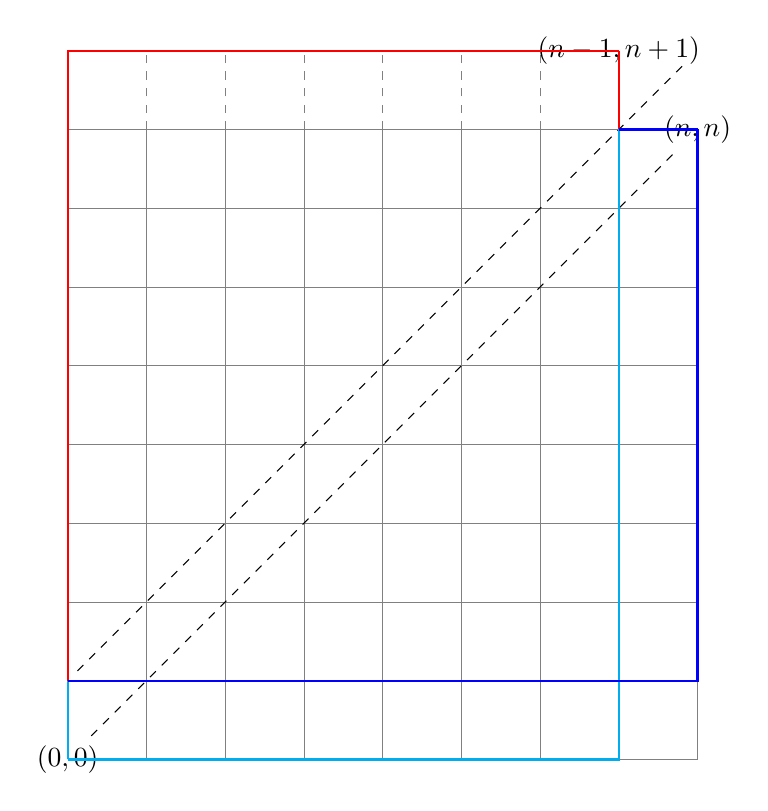
\begin{tikzpicture}
  \draw[help lines] (0,0) grid (8,8);
  \draw[help lines, dashed] (0,8) grid (7,9);

  \node (00) [] {$(0,0)$};
  \node (01) [] at (0,1) {};
  \node (nn) [] at (8,8) {$(n,n)$};
  \node (nn1) [] at (8,9) {};
  \node (n1n1) [] at (7,9) {$(n-1, n+1)$};

  \draw [dashed] (00) to (nn);
  \draw [dashed] (01) to (nn1);

  \draw[thick, cyan] (0,0) -- (7,0) -- (7,8);
  \draw[thick, red] (7,8) -- (7,9);
  \draw[thick, blue] (7,8) -- (8,8);

  \draw[thick, cyan] (0,0) -- (0,1);
  \draw[thick, red] (0,1) -- (0,9) -- (7,9);
  \draw[thick, blue] (0,1) -- (8,1) -- (8,8);
\end{tikzpicture}
\end{document}

